\documentclass{article}

\usepackage{a4wide,amsmath,amssymb,fancyhdr,graphicx,tabularx,xspace, algorithmic,amsmath,dsfont}

\pagestyle{fancy}
\chead{}
\lhead{TU Eindhoven}
\rhead{Algorithms (2IL15) --- Homework Exercises}
\cfoot{\thepage}
\lfoot{}
\rfoot{}

%to include IPE/pdf correctly
\expandafter\ifx\csname pdfoptionalwaysusepdfpagebox\endcsname\relax\else
\pdfoptionalwaysusepdfpagebox5
\fi

%comments command
\newcommand{\complain}[1]{\begin{quotation} {\sf *** #1 ***} \end{quotation}}


%
% Macros
%


\newcommand{\Reals}{{\Bbb R}}
\newcommand{\Nats}{{\Bbb N}}
\newcommand{\Ints}{{\Bbb Z}}


\newcommand{\C}{\ensuremath{\mathcal{C}}}
\newcommand{\E}{\ensuremath{\mathcal{E}}}
\newcommand{\F}{\ensuremath{\mathcal{F}}}
\newcommand{\G}{\ensuremath{\mathcal{G}}}
\newcommand{\U}{\ensuremath{\mathcal{U}}}

\newcommand{\tree}{\ensuremath{\mathcal{T}}}
\newcommand{\node}{\nu}
\newcommand{\lchild}{\mathrm{lc}}
\newcommand{\rchild}{\mathrm{rc}}
\newcommand{\size}{\mathit{size}}
\newcommand{\leaf}{\mu}
\newcommand{\mylist}{{\cal L}}
\newcommand{\myroot}{\mathit{root}}
\newcommand{\key}{\mathit{key}}
\newcommand{\bd}{\partial}





\newcommand{\eps}{\varepsilon}
\newcommand{\ol}{\overline}
\renewcommand{\leq}{\leqslant}
\renewcommand{\geq}{\geqslant}



\newcommand{\pr}[1]{\Pr[#1]}
\DeclareMathOperator{\expectation}{E}
\newcommand{\expt}[1]{\expectation[#1]}
\newcommand{\events}[1]{\mbox{Events}(#1)}
\newcommand{\rank}{\mathit{rank}}
\newcommand{\result}{\mathit{result}}
\newcommand{\piv}{\mathrm{piv}}
\newcommand{\myexp}{\mathrm{exp}}
\newcommand{\best}{\mathrm{best}}
\newcommand{\worst}{\mathrm{worst}}
\newcommand{\dest}{\mathit{dest}}
\newcommand{\dist}{\mathit{distance}}
\newcommand{\weight}{\mathit{weight}}
\newcommand{\alg}{{\sc Alg}\xspace}

\newcommand{\start}{\mathit{start}}
\newcommand{\myend}{\mathit{end}}
\newcommand{\free}{\mathit{free}}

\newcommand{\etal}{{\emph{et al.}\xspace}}
%%
% Theorem-Like Environments
%
\newtheorem{defin}{Definition}
  \newenvironment{mydefinition}{\begin{defin} \sl}{\end{defin}}
\newtheorem{theo}[defin]{Theorem}
  \newenvironment{mytheorem}{\begin{theo} \sl}{\end{theo}}
\newtheorem{lem}[defin]{Lemma}
  \newenvironment{mylemma}{\begin{lem} \sl}{\end{lem}}
\newtheorem{propo}[defin]{Proposition}
  \newenvironment{myproposition}{\begin{propo} \sl}{\end{propo}}
\newtheorem{coro}[defin]{Corollary}
  \newenvironment{corollary}{\begin{coro} \sl}{\end{coro}}
%\newtheorem{obse}[defin]{Observation}
%  \newenvironment{observation}{\begin{obse} \sl}{\end{obse}}
%\newtheorem{rem}[defin]{Remark}
%  \newenvironment{remark}{\begin{rem} \rm}{\end{rem}}


\newenvironment{myproof}{\emph{Proof.}}{\hfill $\Box$ \medskip\\}

\newcounter{rcounter}
\newenvironment{rlist}%
{\begin{list}{A.1-\arabic{rcounter}}{\usecounter{rcounter}}}{\end{list}}
\newcounter{rcountermem}

%%%%%%%%%%%%%%%%%%%%%%%%%%%%%%%%%%%%%%%%%%%%%%%%%%%%%%%%%%%%%%%%%%%%%

\title{}
\author{Mart Pluijmaekers}
\date{3-12-2012}


%%%%%%%%%%%%%%%%%%%%%%%%%%%%%%%%%%%%%%%%%%%%%%%%%%%%%%%%%%%%%%%%%%%%%%%%%%%

\begin{document}

\section*{Algorithms (2IL15): Homework Set A}

\subsection*{Single-source shortest paths}
\begin{itemize}
\item[(1)] Lets assume that the claim does not hold, then we needed to find a graph ($G'$) which is formed in such a way that it breaks the claim. This graph needs to have a vertex which is connected to $G'$ but, is not efficiently relaxable even if we know the order in which to relax all edges of $E'$. That would mean that there does not exist a ``simple'' path from the source node to this node. Simple meaning, a path for which it is easy to calculate the sum of weights. Since we know that weight sums can be easilly calculated, we know that every path is one of these simple paths and thus we know that the original claim holds. \\

We can show that if we take any graph $G=(V,E)$ we can choose a subset of the edges ($E'$) such that the claim holds. We can even write an algorithm for it. If we take Dijkstra's algorithm (for example) and take a graph in which the vertices can remember which edge was used to relax them the last time they were relaxed. After Dijstra is run, we can now retrieve all the edges stored in every vertex. This subset only contains the edges which build op all of the shortest paths. This graph is obviously a tree, since every vertex only stored the last edge to relax it and this this vertex is only connected to one other vertex (where this vertex is on the receiving end of a edge). The number of elements in $E'$ is equal to $|V|-1$ since all vertices only have one incoming edge.\\

Since this subset of edges contains all edges which minimize the total weight of all paths  we know we have the shortest possible paths, if we then insert this subset in a modified version of Dijkstra (for example) which relaxes only those edges, we are always finished in linear time, since $\#E'=|V|-1$.


\item[(2)]  Since we know that $v$ is not reachable from $s$ we have 2 distinct cases, either v is connected to the rest of $G$ trought edges starting in $v$, or $v$ does not have any edges. (assumption: $v \ne s$)

\begin{itemize}

\item[$v$ has no edges] If $v$ has no edges then ony \emph{Initialize-Single-Source(G,s)} is run and thus $d[v]=\infty$.
\item[$v$ has edges] If $v$ has (outgoing) edges, we have 3 distinct cases, either the weight is positive, negative or zero, but since $\infty + x= \infty , x \in \mathds{R}$ we treath these 3 cases together, since we know that the $d[v]=\infty$ after \emph{Initialize-Single-Source(G,s)} is run, we can now see that when \emph{Relax(u,v)} is executed, the guard in the if statement will never hold, since $d[v]$ is either $\infty$ or possibly a element from $\mathds{R}$. Thus $d[v]=\infty$

\end{itemize}

We have shown that for both cases it holds that $d[v]=\infty$.

\item[(3)] It depends on the way the edges are relaxed, but if we take the most stupid way possible, we can always get a correct awnser after $a+b$ rounds of relaxations, this is because the maximal length of a path is $a+b$. The most stupid way would be if we started relaxing all the edges starting from the vertex furthest away from the source and worked our way back. Because we then would only calculate acurate paths for length equal to the pass we are currently at. For example if we are in the 3 round of relaxations, we would have only relaxed all paths of length 3 correctely. Thus the maximal number of relaxations neccesary is $a+b$

\item[(4)] \begin{itemize}
\item[(i)] The algorithm now computes the Single-source shortest paths problem from both $s$ and $t$, in other words, it computes the smallest distance from $s$ or $t$ to any other vertex.
\item[(ii)] \textbf{invariant:} At start of each iteration of while-loop: $d(v) = \delta(s,v)$ or $d(v) = \delta(t,v)$  for all $v$ in $S$. \\

\textbf{initialization:} \\
$S\gets \emptyset$, so invariant holds before first iteration.


\textbf{maintenance:} \\
must prove $d(u) =\delta(s,u)$ or $d(u)=\delta(t,u)$ for selected vertex $u$, let $(v,u)$ be the chosen edge.  \\

For every vertex, on path from $s$ or $t$ to $u$, we have to check whether or not every element is on the shortest path. \\

Let $x_1,x_2$ be elements on the paths from $s$ and $t$ to $u$ respectively. Then $y_1,y_2$ be the next vertices on the paths, then we have 2 distinct cases. \\

\textbf{case: $y_1$ or $y_2 = u$:} We are done, $(x,y_1)$ or $(x,y_2)$ has been relaxed so $d(u)=$min$(\delta(s,u),\delta(t,u))$ \\

\textbf{case: $y_1$ or $y_2 \ne u$:} 
Then it holds that $d(u) \le d(y_1) = \delta(s,y_1) \le \delta(s,u)$ or $d(u) \le d(y_2) = \delta(t,y_2) \le \delta(t,u)$, also $d(u) \le \delta(s,u)$ or $d(u) \le \delta(t,u)$ by property of Relax. Since these statements hold for either $s$ or $t$, we know that $d(u)=\text{min}(\delta(s,u),\delta(t,u))$.

\end{itemize}
\end{itemize}

\subsection*{All-pairs shortest paths}
\begin{itemize}
\item[(1)] No, we do not have to change the edge weights, since we know we do not have any negative weight cycles, we can simply run dijkstra's algorithm. If we were to change the edge weights, we can find  the lowest edge weight and add its absolute value to every edge weight, so we end up with edge weights which are $\ge 0$.

\item[(2)]
\begin{algorithmic}[1]
\STATE{Bounded-Length-Negative-Cycle(G, k)}
\FOR{each vertex $v$ in $V$}
\FOR{each edge $(v,u)$ in $E$}
\IF{Check($v,k-1,w[v,u]$)}
\RETURN{\TRUE}
\ENDIF
\ENDFOR
\ENDFOR
\RETURN{\FALSE}
\end{algorithmic} 
\bigskip
\begin{algorithmic}[1]
\STATE{Check($cu,k,c,e$)}
\IF{$k<0$} \RETURN{\FALSE}\ENDIF
\IF{$e=cu \wedge c<0$} \RETURN{\TRUE}\ENDIF
\FOR{each edge $(e,v)$ in $E$}
\IF{Check($cu,k-1,c+w[e,v],v$)}
\RETURN{\TRUE}
\ENDIF
\ENDFOR
\RETURN{\FALSE}
\end{algorithmic}

\end{itemize}

\textbf{Correctness:}
If we take a look at the algorithm we can see that for every vertex it tries to compute whether or not there is a path with length at most $k$ back to itself and that the total weight of this graph is negative. I'll argue the correctness for a single arbitrary vertex ($v$).\\

After the selection of $v$ we start iterating over each of the edges which originate in $v$, for each of these vertices ($u$) we do the same step recursively (for at most $k$ times) and keep checking whether we end up in $v$ or not. Because we keep a refrence to the current path weight, we know at all times the sum of the edge weights and thus can check if a found cycle has a negative weight or not. \\


\textbf{Running-time:}
For the running time analysis we again have to take a look at the algorithm, we can see that \emph{Bounded-Length-Negative-Cycle(G, k)} holds (nested) loops. The first loop iterates over all of the Vertices, thus this loop has $n$ iterations. The inner loop iterates over edges which is atmost $|V|-1$, assuming that there is no edge from a given Vertex to itself. The function which is called by this loop does exactely the same thing while. Since we have the guard on the second line of \emph{Check($cu,k,c,e$)} which makes sure that we only recurse for $k$ times we get a running-time of:
$|V| * k * (|V|-1)=|V|*(|V|-1)*k<|V|*|V|*k$, let $n=|V|$ then we have a running time of: $n*n*k=n^2k$. So the algorithm runs  $O(n^2k)$ time which is less then $O(n^3k)$. \\

(note all other lines (everything except the loops) in both function has a running time of $O(1)$.)

\subsection*{Max-Flow}
\begin{itemize}
\item[(1)] \begin{itemize}
\item[(i)] If we look at the residual network and then specifically to the yellow node, we can see that when we diverge the flow from the yellow node towards the node to its right, to the node above the yellow node, we can free up a slot on the righthand side of the network. Which allows us to enhance the total flow using the freed up slot. (This will flow from the source all the way to the right and then directely to the sink.)

\begin{center}\includegraphics[scale=0.4]{flow0}\\Residual network\end{center}

\item[(ii)] If we take the enhanced flow described in the previous exercise, we can create a cut over the elements connected to the sink. We can count that the flow going into these nodes is equal to: 9 and the flow flowing out of these two nodes (and into the sink) is also equal to 9. Note that the possible maximal flow is also equal to 9 since, the capacity of both of the edges leading into the sink is 6 and 3. So the one of the possible cuts is over the sink.

\end{itemize}

\item[(2)] \begin{itemize}
\item[(i)] This claim does not hold because there is a possibility that the flow is maximal, while there is still flow flowing back into the source. See this example:

\begin{center}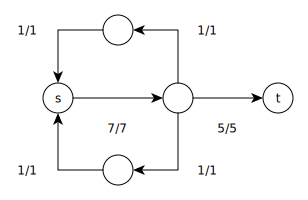
\includegraphics[scale=0.5]{backflow}\end{center}

\item[(ii)] This claim does hold, since we can clearly see from the previous example that whenever we have a graph, with flow flowing back into the source, it does not matter for the maximal flow over a cut whether these flows are $0$ or not.

\end{itemize}

\item[(3)] If we look at the flow network depicted in the image, we see the availability of blood of a given type flows from the source and blood needed flows to the sink. All edges with no capacity specified, have infinite capacity. In order to decide what patient gets what type of blood we have to look at the flow flowing into the sink. If we had previously given every ``flow unit'' a unique id and we look at which vertex on the left hand side it flows through we know what type of blood we have to give this patient.
\begin{center}\includegraphics[scale=0.4]{flow2}\end{center}

The flow network works as follows. All needed blood is on the left hand side and all available blood is on the right hand side (as capacities). The connections in the middle all have infinite capacity. The connections in the middle depict which blood type can receive which blood types, obviously every bloodtype can receive its own type, but everyone can receive O and AB can receive from blood from any bloodtype. This flow network is calculatable by any algorithm, since it does not require any specifics.

\end{itemize}


\end{document} 